\chapter{METODOLOGI}
\label{chap:metodologi}

% Ubah bagian-bagian berikut dengan isi dari desain dan implementasi

% Penelitian ini dilaksanakan sesuai \lipsum[1][1-5]
% \section{Data dan Peralatan}
% Adapun tata pendukung berupa data dan peralatan yang digunakan dalam pelaksanaan penelitian tugas akhir ini adalah sebagai berikut:

% \noindent \textbf{Data}\\
% Data yang akan digunakan merupakan kumpulan citra berukuran 640px x 480px. Kumpulan citra ini didapat melalui ekstraksi video yang berisi pengucapan bahasa isyarat BISINDO. Kumpulan citra ini dibuat secara mandiri oleh penulis menyesuaikan dengan kebutuhan kosakata isyarat dan kosakata tambahan yang dibutuhkan.

% \noindent \textbf{Peralatan}\\
% Adapun peralatan yang digunakan dalam penelitian tugas akhir ini adalah sebagai berikut:

% \begin{itemize}
%   \item Visual Studio Code
%   \item Anaconda
%   % \item Jetson Nano B01 Developer Kit
%   \item Intel Next Unit Computing (NUC) 
%   \item Webcam
%   \item Speaker
%   \item Laptop
% \end{itemize}

Tugas akhir ini akan dilaksanakan sesuai dengan desain sistem beserta implementasinya yang akan dibahas pada bab ini. Desain sistem ini merupakan konsep dasar perancangan dan pembuatan program pada tugas akhir ini. Desain sistem ini direpresentasikan dalam bentuk blok diagram yang diselesaikan secara bertahap dan menyeluruh.

\section{Metode yang Digunakan}

% Penelitian tugas akhir ini dilaksankaan sesuai dengan desain sistem yang tertera pada bab ini. Desain sistem yang dibuat merupakan konsep dari perancangan dan implementasi penelitian ini. Blok diagram pada gambar \ref{fig:blockdiagrammethod} merupakan serangkaian alur yang diikuti dalam pelaksanaan dan pengimplementasian tugas akhir ini.

Adapun tugas akhir ini merupakan pengembangan dari teknologi visi komputer yang kemudian diimplementasikan pada Intel \emph{Next Unit Computing} (NUC). Secara umum, pelaksanaan tugas akhir ini didasari oleh blok diagram yang dapat dilihat pada gambar \ref{fig:blockdiagrammethod}.

\begin{figure}[H]
  \centering

  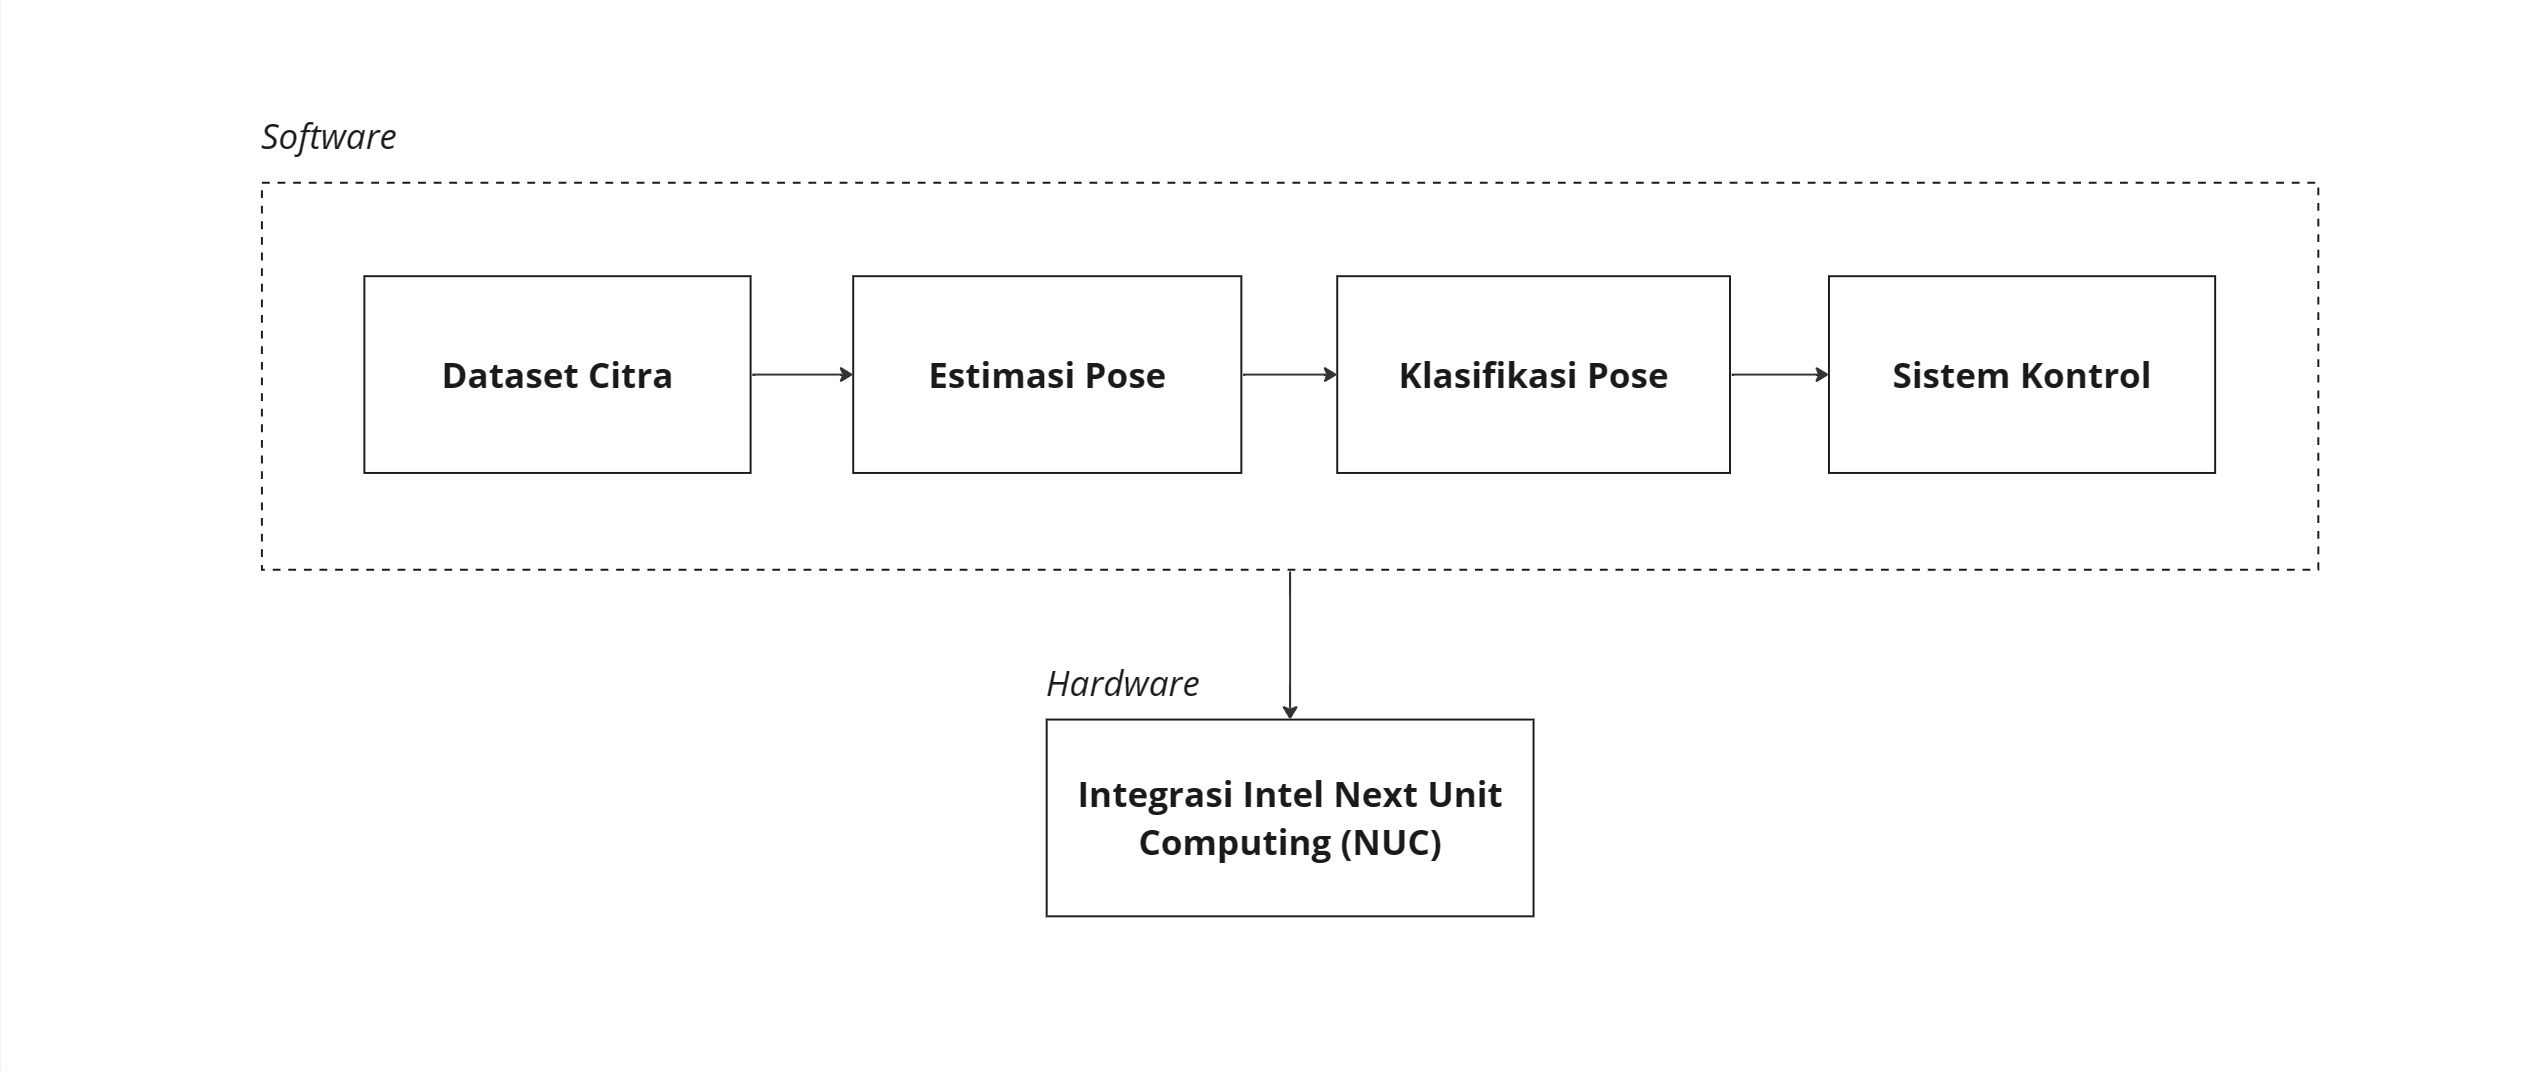
\includegraphics[scale=0.16]{gambar/bab3-block-diagram-nuc.jpg}

  \caption{Blok diagram metodologi}
  \label{fig:blockdiagrammethod}
\end{figure}

\subsection{Dataset Citra}
\label{sec:metodologidataset}

% Dataset yang akan digunakan pada tugas akhir ini merupakan kumpulan citra yang berbentuk sekuensial atau berurutan. Pengambilan dataset dilakukan di dalam ruangan tertutup dengan jarak bervariasi antara 1 - 2 meter dari kamera laptop dengan posisi setengah berdiri (dari pinggang hinga kepala). Data video yang didapatkan kemudian diproses melalui \textit{library} Python OpenCV sehingga dihasilkan citra. Pengambilan citra dilakukan sebesar 30 \textit{frame per second} (FPS) sehingga dalam satu detik terdapat 30 citra. Pembatasan FPS ini diharapkan dapat memberikan hasil yang stabil dan konsisten dalam pengambilan citra. Citra akan disimpan pada laptop secara lokal sehingga dapat diamati nantinya apakah gerakan bahasa isyarat yang dilakukan telah benar atau tidak dan menghasilkan dataset yang baik digunakan dalam pembuatan model klasifikasi. Dapat dilihat pada gambar \ref{fig:datasetMethod} akan dihasilk total 30 citra. Perlu diperhatikan bahwa ukuran dari citra yang akan digunakan pada tugas akhir ini adalah sebesar 640px x 480px

Dataset yang akan digunakan dalam pelaksanaan tugas akhir ini merupakan kumpulan citra dalam bentuk sekuensial atau berurutan. Pengambilan dataset akan dilakukan di dalam ruangan tertutup dengan jarak antara kamera dengan penulis bervariasi antara 1 - 2 meter dari kamera laptop. Posisi penulis terhadap kamera adalah dalam keadaan berdiri. Akan didapatkan data berupa video melalui bantuan \emph{library} OpenCV. Video yang diambil merupakan kumpulan dari total 30 \emph{frame} atau citra sebesar 640 pixel x 480 pixel. Pembatasan ini ditujukan untuk membuat dataset dengan hasil yang stabil dan konsisten dalam semua gerakan isyarat yang dilakukan. Dataset akan disimpan pada laptop secara lokal untuk nantinya diamati apakah gerakan isyarat BISINDO yang dilakukan telah benar dan menunjukkan keunikan dari masing - masing kosakata. Hal ini penting diamati untuk menghasilkan model LSTM dengan performa klasifikasi yang baik. Contoh satu data yang merepresentasikan gerakan isyarat untuk kosakata "nama" dapat dilihat pada gambar \ref{fig:datasetMethod}.

\begin{figure}[H]
  
  \centering

  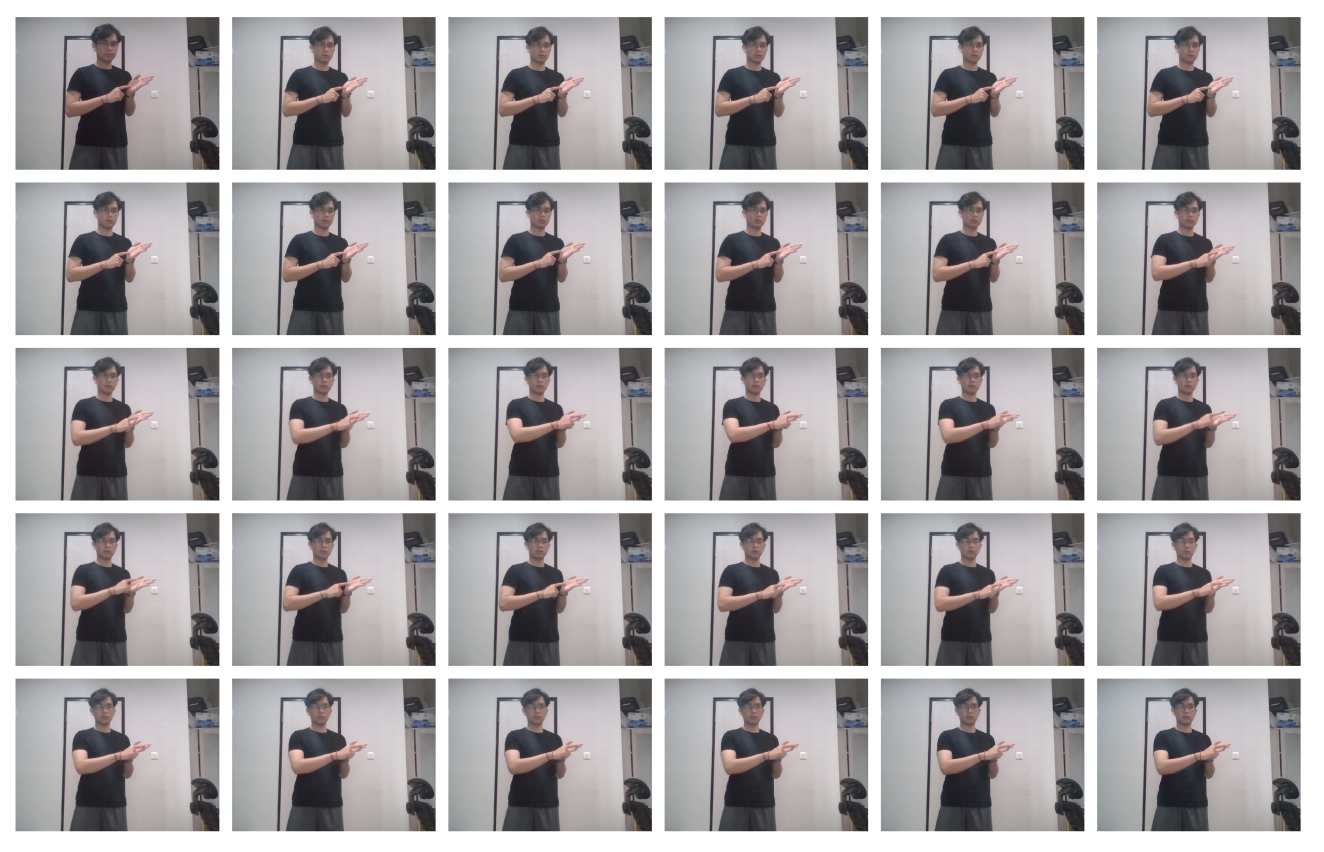
\includegraphics[scale=0.5]{gambar/isyarat-clear-nama.png}

  \caption{Dataset kosakata "nama"}
  \label{fig:datasetMethod}
\end{figure}

Adapun bahasa isyarat yang akan digunakan pada tugas akhir ini meliputi 6 kosakata isyarat BISINDO yang memiliki konteks kalimat yang umum digunakan sehari – hari. Nantinya untuk setiap kosakata tersebut akan disimpan sebanyak 30 jumlah data dengan masing - masing data terkumpul sebanyak 30 \emph{frame}. Kosakata yang akan digunakan adalah sebagai berikut:

\begin{longtable}{|c|c|c|c|}
  \caption{Kosakata BISINDO}
  \label{tb:kosakataBISINDO}                                   \\
  \hline
  \rowcolor[HTML]{C0C0C0}
  \textbf{No} & \textbf{Kelas} & \textbf{Jumlah Data} & \textbf{Jumlah \emph{Frame}}\\
  \hline
  1            & Maaf                       & 30            & 30\\
  2            & Tolong                     & 30            & 30\\
  3            & Saya                       & 30            & 30\\
  4            & Nama                       & 30            & 30\\
  5            & Rumah                       & 30            & 30\\
  6            & Siapa                       & 30            & 30\\
  \hline
\end{longtable}

% Digunakan tambahan 3 buah isyarat tambahan di luar isyarat BISINDO untuk mempermudah kontrol sistem penerjemah. Isyarat tersebut meliputi isyarat mulai (\textit{start}), isyarat \textit{standby}, isyarat hapus kata (\textit{delete}), dan isyarat terjemah (\textit{translate}).  

Dalam mempermudah kontrol sistem penerjemah, digunakan 3 gerakan isyarat tambahan di luar gerakan isyarat BISINDO.  Isyarat tersebut meliputi isyarat \textit{standby}, isyarat hapus kata (\textit{delete}), dan isyarat terjemah menjadi suara (\textit{translate}).  Untuk setiap gerakan isyarat kontrol juga memiliki jumlah data yang sama dengan gerakan isyarat BISINDO, yaitu 30 data dengan 30 \emph{frame} pada setiap datanya.

\begin{longtable}{|c|c|c|c|}
  \caption{Isyarat Kontrol Tambahan}
  \label{tb:isyaratkontrol}                                   \\
  \hline
  \rowcolor[HTML]{C0C0C0}
  \textbf{No} & \textbf{Kelas} & \textbf{Jumlah Data} & \textbf{Jumlah \emph{Frame}}\\
  \hline
  1            & \textit{Standby}                       & 30             & 30 \\
  2            & \textit{Translate}                     & 30             & 30 \\
  3            & \textit{Delete}                        & 30             & 30 \\
  \hline
\end{longtable}

\subsection{Estimasi Pose}

\begin{figure}[H]
  \centering

  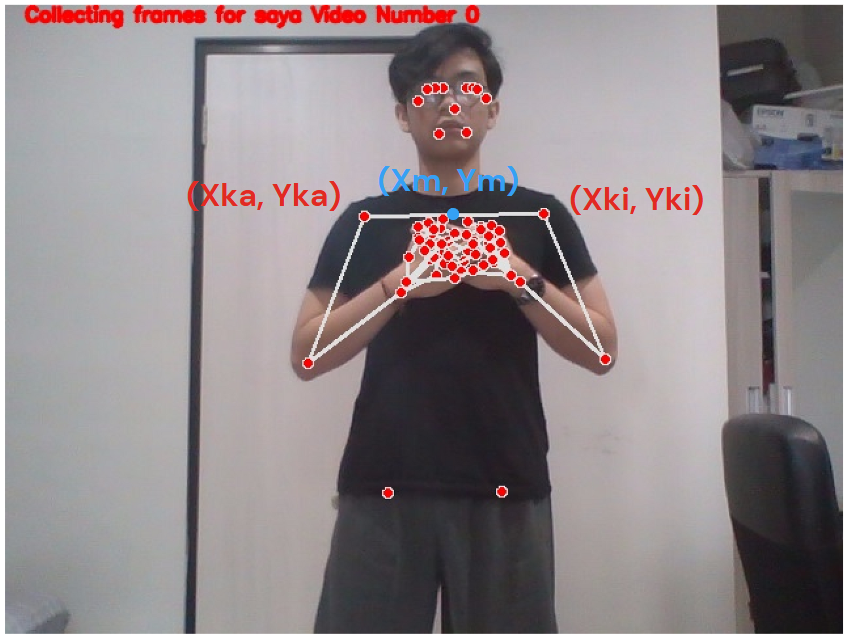
\includegraphics[scale=0.6]{gambar/bab3-estimasi-pose.png}

  \caption{Estimasi pose pada citra}
  \label{fig:poseEstimationMethod}
\end{figure}

Untuk setiap citra pada 30 data yang telah dilakukan estimasi pose dengan bantuan \textit{framework} MediaPipe. \textit{Framework} ini dapat melacak titik – titik bagian tubuh atau \textit{landmark} menggunakan model yang disediakan. Model MediaPipe yang akan digunakan adalah MediaPipe pose dan MediaPipe hand. Dalam pembentukan isyarat BISINDO, bagian tubuh yang bergerak adalah bagian tangan dan lengan. Melalui MediaPipe hand akan dilakukan ekstraksi untuk 21 \textit{landmark} pada bagian tangan, sehingga total \textit{landmark} untuk tangan kanan dan kiri adalah 42 \textit{landmark}. Kemudian melalui MediaPipe pose akan dilakukan ekstraksi pada bagian bahu sampai lengan sehingga \textit{landmark} yang akan digunakan hanya pada posisi 11 hingga 22 sehingga total \textit{landmark} untuk bagian tubuh adalah 12 \textit{landmark}. Untuk setiap \textit{landmark} yang didapatkan akan digunakan koordinat x dan y saja (koordinat z dan \textit{visibility} tidak digunakan). Hal ini berguna demi menghasilkan model akhir yang memiliki kemampuan untuk invarian terhadap skala (jarak kamera tidak mempengaruhi estimasi pose) dan invarian terhadap rotasi (adanya rotasi tidak mempengaruhi koordinat yang digunakan). Hal ini juga dilakukan demi melakukan reduksi dimensi sehingga mengurangi resiko \textit{overfitting} dan dapat mempercepat performa model. Nantinya, untuk setiap citra yang akan diproses pada MediaPipe akan menghasilkan total 42 koordinat dari \textit{landmark} tangan kanan, 42 koordinat dari \textit{landmark} tangan kiri, dan 24 koordinat dari \textit{landmark} pose.Hal ini dapat dilihat pada gambar \ref{fig:poseEstimationMethod}, \textit{landmark} yang akan digunakan hanyalah \textit{landmark} yang saling terhubung (ditandai dengan garis putih). Sedangkan \textit{landmark} yang hanya berbentuk titik saja tidak akan digunakan dan tidak akan diambil data koordinatnya. Data koordinat \textit{landmark} yang berbentuk array multidimensi kemudian akan diproses melalui \textit{library} Numpy dengan menggunakan fungsi concatenate menjadi satu dimensi saja untuk mempermudah pada klasifikasi pose pada tahap \textit{training} data.

\subsubsection{Normalisasi Data}
Keseluruhan data koordinat yang didapatkan melalui estimasi pose menggunakan MediaPipe akan melalui proses normalisasi. Normalisasi data dilakukan demi mengatasi adanya \textit{scale invariant} dan \textit{position invariant}. \textit{Scale invariant} dalam konteks tugas akhir ini adalah kemampuan model dalam mengklasifikasikan data bahasa isyarat yang dilakukan oleh berbagai macam pengguna yang memiliki bentuk tubuh yang berbeda - beda. Selain itu, \textit{scale invariant} juga menyebabkan jarak pengguna dengan kamera tidak mempengaruhi proses klasifikasi model. \textit{Position invariant} dalam konteks tugas akhir ini adalah kemampuan model dalam mengklasifikasikan data bahasa isyarat dalam berbagai posisi pengguna terhadap kamera (dengan catatan bahwa posisi tangan dan bahu dapat terlihat jelas ketika pengguna melakukan gerakan isyarat).

\begin{equation}
  \label{eq:shouderWidthNorm}
  w = \sqrt{(x_{ka} - x_{ki})^2 + (y_{ka} - y_{ki})^2}
\end{equation}

\begin{equation}
  \label{eq:shoulderMidpointNorm}
  x_m = \frac{x_{ka} + x_{ki}}{2} ; \\
   y_m = \frac{y_{ka} + y_{ki}}{2}
\end{equation}

\begin{equation}
  \label{eq:normalization}
  x'_i = \frac{x_i - x_m}{w} ;  \\
   y'_i = \frac{y_i - y_m}{w}
\end{equation}

Dalam melakukan proses normalisasi, terlebih dahulu didapatkan panjang dari bahu dengan menggunakan rumus jarak \textit{Euclidian}. Rumus ini akan menghitung kuadrat selisih antara koordinat x dan y antara \textit{landmark} bahu kanan dan kiri. Hasil dari kedua operasi tersebut kemudian dijumlahkan dan dihitung akar kuadratnya. Perhitungan jarak \textit{Euclidian} dapat dapat dilihat pada rumus \ref{eq:shouderWidthNorm}. Untuk mendapatkan titik tengah dari \textit{landmark} bahu, dilakukan dengan menjumlahkan masing - masing koordinat x dan y dari bahu kanan dan kiri, kemudian dibagi dengan 2. Proses ini dapat dilihat pada rumus \ref{eq:shoulderMidpointNorm}.

Normalisasi data akan dilakukan dengan melakukan pengurangan terhadap setiap koordinat \textit{landmark} dengan koordinat titik tengah dari bahu dan diakhiri dengan pembagian dengan panjang dari bahu yang telah dihitung sebelumnya. Hal ini dapat dilihat pada rumus \ref{eq:normalization}. Perlu diketahui bahwa pada perumusan diatas, $w$ adalah panjang bahu, $x_{ka}$ adalah koordinat x bahu kanan, $y_{ka}$ adalah kooridnat y bahu kanan, $x_{ki}$ adalah koordinat x bahu kiri, $y_{ki}$ adalah kooridnat y bahu kiri, $x'_i$ adalah koordinat x yang telah dinormalisasi, dan $y'_i$ adalah kooridnat y yang telah dinormalisasi.

Nantinya data koordinat yang telah dinormalisasi ini akan disimpan dalam bentuk array dengan bantuan Numpy dan akan digunakan dalam proses \textit{training}. Normalisasi data tidak hanya digunakan dalam proses pembuatan model, tetapi juga nantinya dalam proses klasifikasi bahasa isyarat dengan menggunakan model. Hal ini dilakukan sehingga koordinat - kooridnat yang diproses adalah homogen dan menghindari adanya \textit{noise} atau \textit{error}.

\subsection{Klasifikasi Pose}
\label{sec:metodologipose}

Dalam melakukan klasifikasi terhadap pose atau gerakana isyarat yang dilakukan, digunakan model LSTM dengan bentuk sekuensial sehingga dapat menggabungkan serangkaian \emph{layer} untuk menghasilkan model penerjemah bahasa isyarat yang memiliki performa baik. \emph{Layer} pertama merupakan \emph{layer} \textit{TimeDistributed} yang di dalamnya terdapat \emph{layer} \textit{Dense} dengan jumlah unit sebesar 128, fungsi aktivasi '\textit{tanh}' dan input dengan bentuk (30, 108). Penggunaan \textit{TimeDistributed} memastikan bahwa untuk setiap frame (data input) akan diproses secara independen. Pada \emph{layer} ini diimplementasikan \emph{layer} \textit{Dense} yang konsisten pada setiap frame yang ada. Hal ini berguna untuk memastikan bahwa representasi dari data yang dipelajari menjadi konsisten pada setiap iterasi pembelajaran model. Cara kerja \emph{layer TimeDistributed} secara garis besar dapat dilihat pada gambar \ref{fig:layerTimeDistributed}. Perlu diperhatikan bentuk data (30, 108) berarti akan terdapat 30 jumlah frame, dimana untuk setiap frame akan diekstrak total 108 fitur. 108 fitur tersebut merupakan kumpulan dari data koordinat x dan y untuk setiap \emph{landmark} Mediapipe yang digunakan.\emph{Layer} kedua merupakan LSTM pertama yang memiliki jumlah unit 128, return\_sequences=True, fungsi aktivasi '\textit{tanh}', dan input dalam bentuk (30, 108). Pada \emph{layer} ketiga diikuti dengan \emph{layer} Dropout dengan nilai 0.5 untuk menghindari adanya nilai \emph{weight} yang terlalu tinggi. \emph{Layer} selanjutnya, yaitu \emph{layer} keempat merupakan layer LSTM kedua yang memiliki jumlah unit 128, return\_sequences=False, dan fungsi aktivasi '\textit{tanh}'. Pada \emph{layer} kelimat diikuti dengan \emph{layer} Dropout dengan nilai 0.5 untuk menghindari adanya nilai \emph{weight} yang terlalu tinggi. Dapat dilihat bahwa untuk setiap \emph{layer} LSTM memiliki \emph{layer} Dropout untuk menghindari \emph{overfitting} pada model dengan menonaktifkan \emph{neuron} dengan probabilitas sebesar 50\%. 

\begin{figure}[H]
  \centering

  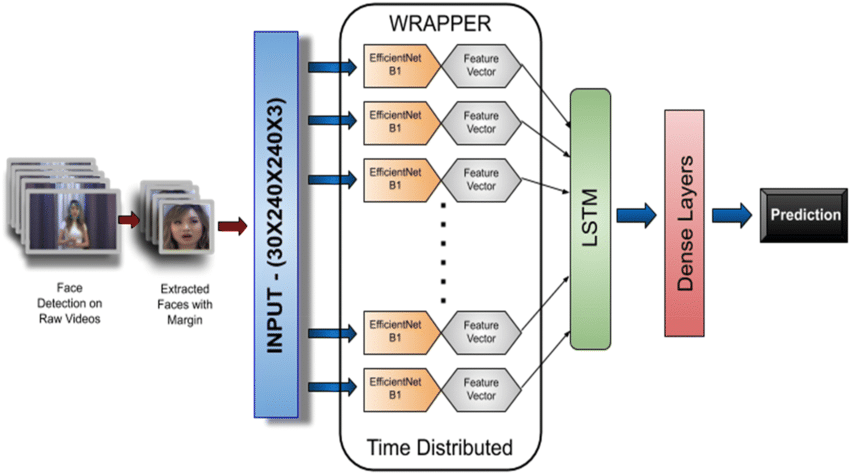
\includegraphics[scale=0.45]{gambar/layer-timedistributed.png}

  \caption{Cara kerja \emph{layer Time Distributed} \parencite{Singh2020}}
  \label{fig:layerTimeDistributed}
\end{figure}

Untuk menyederhanakan kompleksitas dari data output yang diberikan 2 layer LSTM, digunakan \emph{layer} Dense dengan jumlah unit 128 dan fungsi aktivasi 'relu'. Setelah \emph{layer} \textit{Dense}, diberikan \emph{layer} Dropout dengan nilai 0.2 untuk menghindari adanya kelebihan \emph{overfitting} pada model. \emph{Layer} terakhir adalah \emph{layer} \textit{Dense} yang menggunakan fungsi aktivasi '\textit{softmax}'. Jumlah unit di \emph{layer} ini sesuai dengan actions.shape[0], yang berarti jumlah unit sama dengan jumlah aksi atau kategori yang mungkin. Fungsi aktivasi '\textit{softmax}' memastikan bahwa keluaran dari model ini adalah distribusi probabilitas di atas semua kategori yang mungkin, dengan total semua probabilitas sama dengan 1. Model ini kemudian dikompilasi menggunakan \emph{optimizer} Adam, yang dikenal karena performa dan efisiensinya dalam pelatihan jaringan saraf, dan menggunakan \textit{categorical crossentropy} sebagai fungsi \textit{loss} karena ini adalah masalah klasifikasi multi-kelas, dengan metrik akurasi kategorikal untuk memantau performa model selama proses \textit{training}. 

\begin{figure}[H]
  \centering

  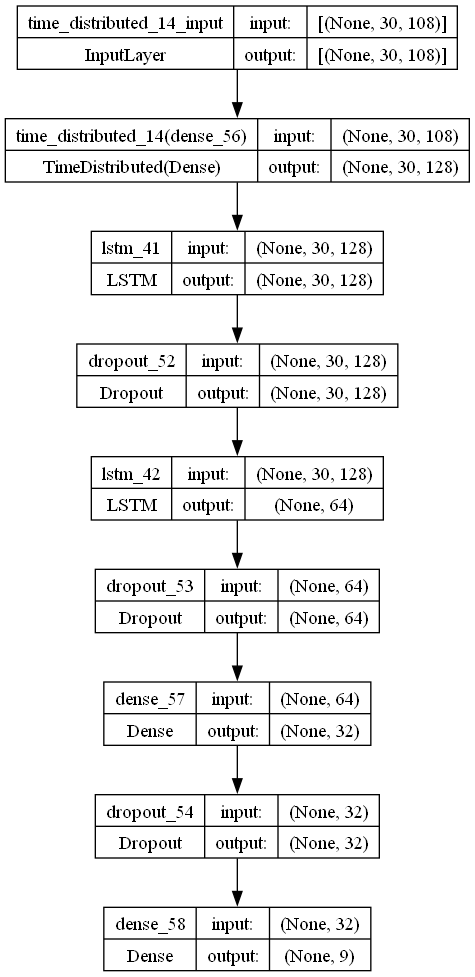
\includegraphics[scale=0.5]{gambar/bab4-uji-model-best-model.png}

  \caption{Model LSTM}
  \label{fig:modelLSTM}
\end{figure}

\subsection{Sistem Kontrol}
\label{sec:metodologisistemkontrol}

Adapun dalam pembuatan tugas akhir ini, sistem kontrol adalah serangkaian proses yang akan mengatur bagaimana nantinya bahasa isyarat akan dideteksi, melakukan penanggulangan terhadap adanya kesalahan pendeteksian, menyatukan berbagai kata dalam bentuk kalimat, penghapusan kosakata, dan penerjemahan kalimat dalam bentuk suara. Penggunaan sistem kontrol ini diharapkan akan memudahkan pengguna dalam menggunakan program penerjemah bahasa isyarat Indonesia (BISINDO). Sistem kontrol akan dibagi menjadi 2, yaitu program deteksi bahasa isyarat dan program pembentukan kalimat.

\subsubsection{Program Deteksi Bahasa Isyarat}

\begin{figure}[H]
  \centering

  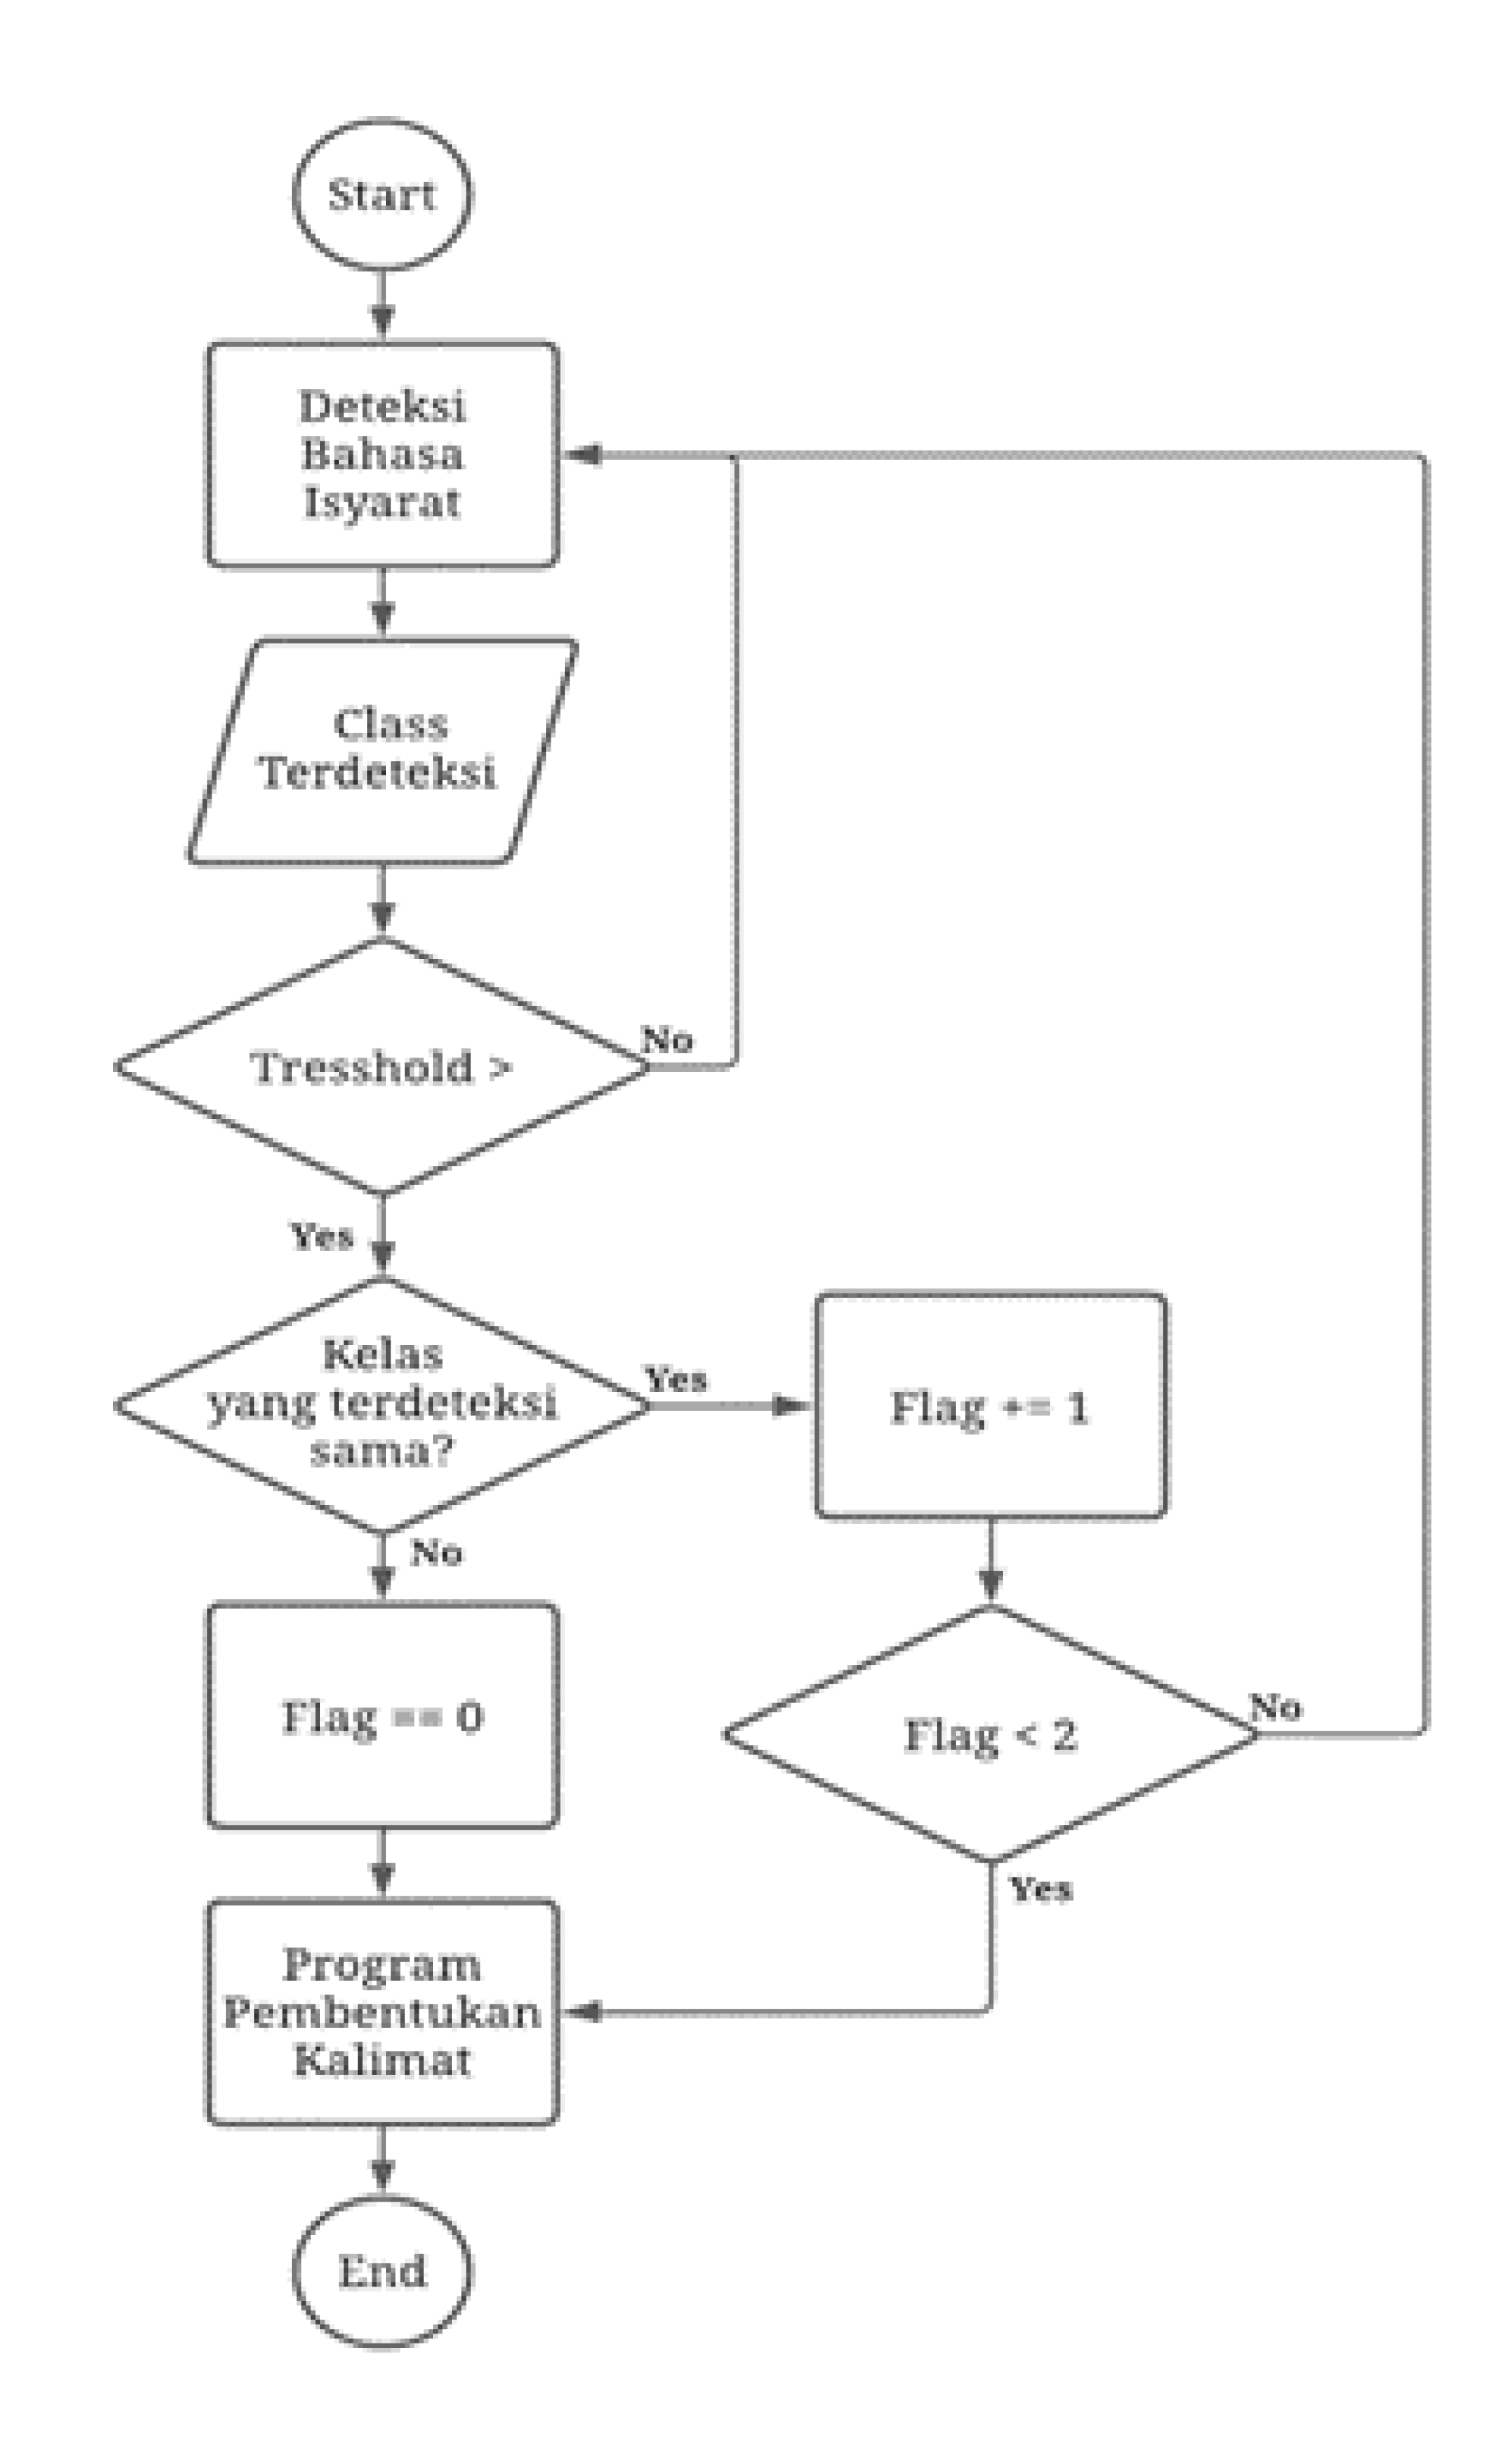
\includegraphics[scale=0.54]{gambar/bab3-flowchart-deteksi.png}

  \caption{Flowchart program deteksi bahasa isyarat}
  \label{fig:flowchartdeteksi}
\end{figure}
Pada program deteksi bahasa isyarat (dapat dilihat pada \ref{fig:flowchartdeteksi}) akan berjalan terlebih dahulu ketika pengguna terdeteksi benar memberikan isyarat start dan pengguna dapat membentuk isyarat yang diinginkan. Kemudian \textit{class} kosakata isyarat yang terdeteksi oleh model akan dipastikan apakah melebihi \textit{threshold} atau ambang batas yang telah ditentukan untuk menghindari adanya kesalahan pembacaan (\textit{error}) dan \textit{noise} dalam pembacaan bahasa isyarat. Apabila dibawah dari \textit{threshold}, maka program akan melakukan pendeteksian kembali bahasa isyarat dari pengguna. Apabila benar diatas dari \textit{threshold} yang ditentukan, maka akan diperiksa apakah \textit{class} yang terdeteksi sama dengan \textit{class} sebelumnya. Apabila terdeteksi sama maka nilai \textit{flag} akan ditambah 1. Nilai \textit{flag} akan diperiksa apakah kurang dari 2, apabila salah maka akan kembali untuk mendeteksi bahasa isyarat dari pengguna. Hal ini dilakukan demi menghindari terjadinya pembacaan isyarat secara berulang kali. Apabila nilai \textit{flag} bernilai 1 atau 0 (nilai awal \textit{flag} adalah 0), maka akan dilanjutkan ke program pembentukan kalimat.

\subsubsection{Program Pembentuk Kalimat}
\begin{figure}[H]
  \centering

  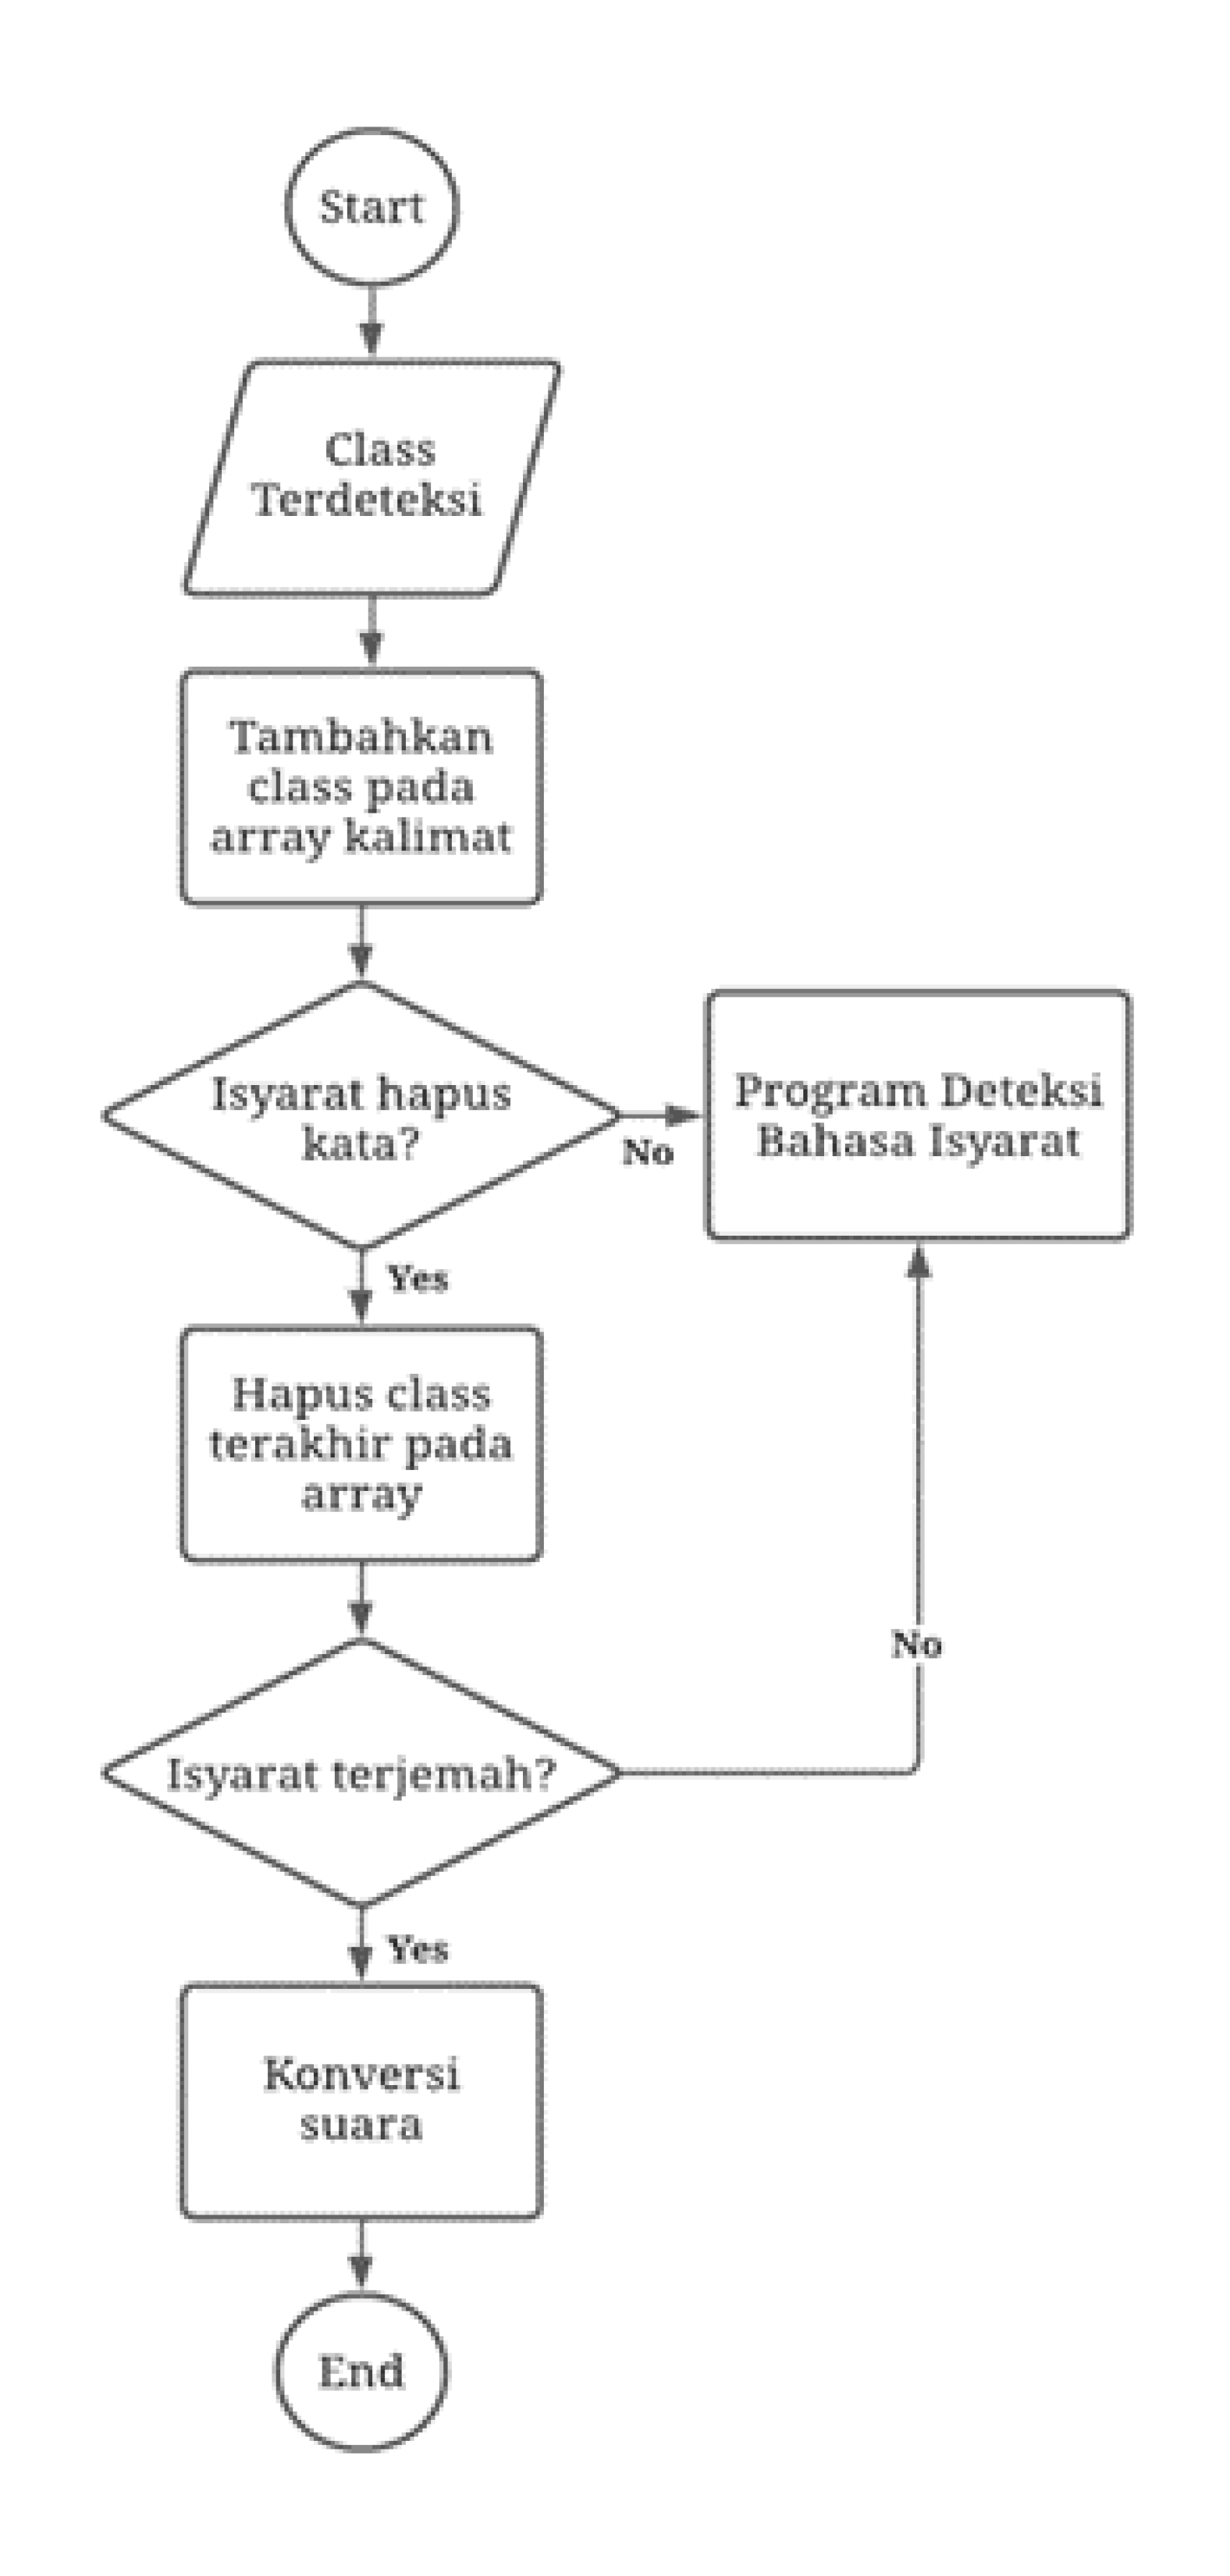
\includegraphics[scale=0.54]{gambar/bab3-flowchart-kalimat.png}

  \caption{Flowchart Program pembentukan kalimat}
  \label{fig:flowchartkalimat}
\end{figure}

Pada program pembentukan kalimat (dapat dilihat pada \ref{fig:flowchartkalimat}), terlebih dahulu \textit{class} kosakata yang terdeteksi akan dimasukkan pada suatu array kalimat dan ditambahkan spasi setelahnya. Hal ini nantinya akan memudahkan pengguna dalam membentuk kalimat yang diinginkan. Kemudian dilakukan pengecekan apakah pengguna melakukan isyarat delete atau hapus, apabila iya maka akan dilakukan penghapusan pada kata terakhir pada array. Apabila tidak maka akan dilanjutkan untuk melakukan pendeteksian bahasa isyarat selanjutnya. Dilakukan juga pengecekan apakah terdapat isyarat translate atau isyarat terjemah, jika iya maka akan dilakukan konversi dari array kalimat yang telah disimpan ke dalam suara dengan memanfaatkan \textit{library} gTTS. Library gTTS merupakan \textit{library} Python yang memiliki kemampuan untuk mengubah suatu string menjadi suara. Nantinya akan dipilih suara dengan aksen Indonesia untuk meningkatkan familiaritas terhadap lingkungan sekitar. Apabila tidak maka akan dilanjutkan untuk melakukan pendeteksian bahasa isyarat selanjutnya.

\subsection{Integrasi Intel Next Unit Computing (NUC)}
\begin{figure}[H]
  \centering

  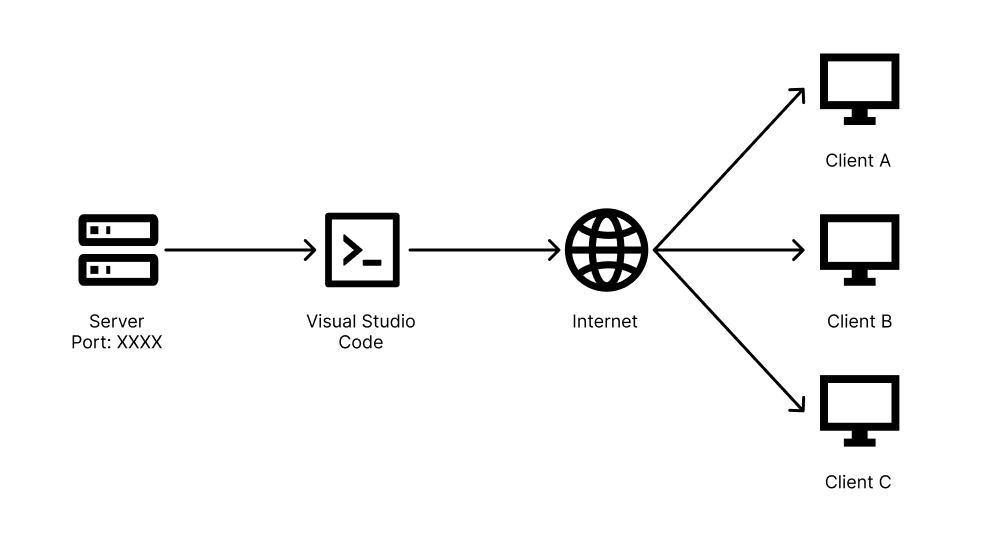
\includegraphics[scale=0.9]{gambar/bab3-path-forwarding.png}

  \caption{Skema integrasi dengan Intel NUC}
  \label{fig:diagrampathforward}
\end{figure}

Sebelum melakukan integrasi, terlebih dahulu perangkat dihubungkan dengan perangkat pendukung seperti monitor, keyboard, mouse, dan speaker. Kemudian, integrasi dengan Intel NUC dilakukan dengan mengakses website penerjemah yang telah terhubung dengan server komputer menggunakan skema \emph{port forwarding} dengan diagram alur yang dapat dilihat pada \ref{fig:blockdiagrammethod}. Server terelebih dahulu mengakses Visual Studio Code untuk menjalankan website penerjemah yang dibuat menggunakan \emph{framework} Streamlit. Akan didapatkan alamat untuk mengakses website tersebut secara lokal (\emph{localhost}), dimana nilai port yang dimiliki oleh server akan diteruskan (\emph{forwarding}) dengan bantuan Ngrok sehingga nantinya akan dapat diakses melalui internet dengan bebas oleh client, yang mana dalam hal ini adalah Intel NUC itu sendiri.

Dapat dilihat pada gambar \ref{fig:tampilanwebsite} bahwa website penerjemah akan mengakses webcam perang\\kat untuk mendapatkan data citra berbentuk video secara \emph{realtime}. Pengguna kemudian dapat melakukan gerakan bahasa isyarat BISINDO di depan webcam. Website penerjemah akan mengekstrak data citra untuk diproses melalui model LSTM yang telah dilatih sebelumnya dan melakukan penerjemahan secara \emph{realtime} sesuai dengan alur program yang telah dijelaskan sebelumnya pada sub bab \ref{sec:metodologisistemkontrol}. 

\begin{figure}[H]
  \centering

  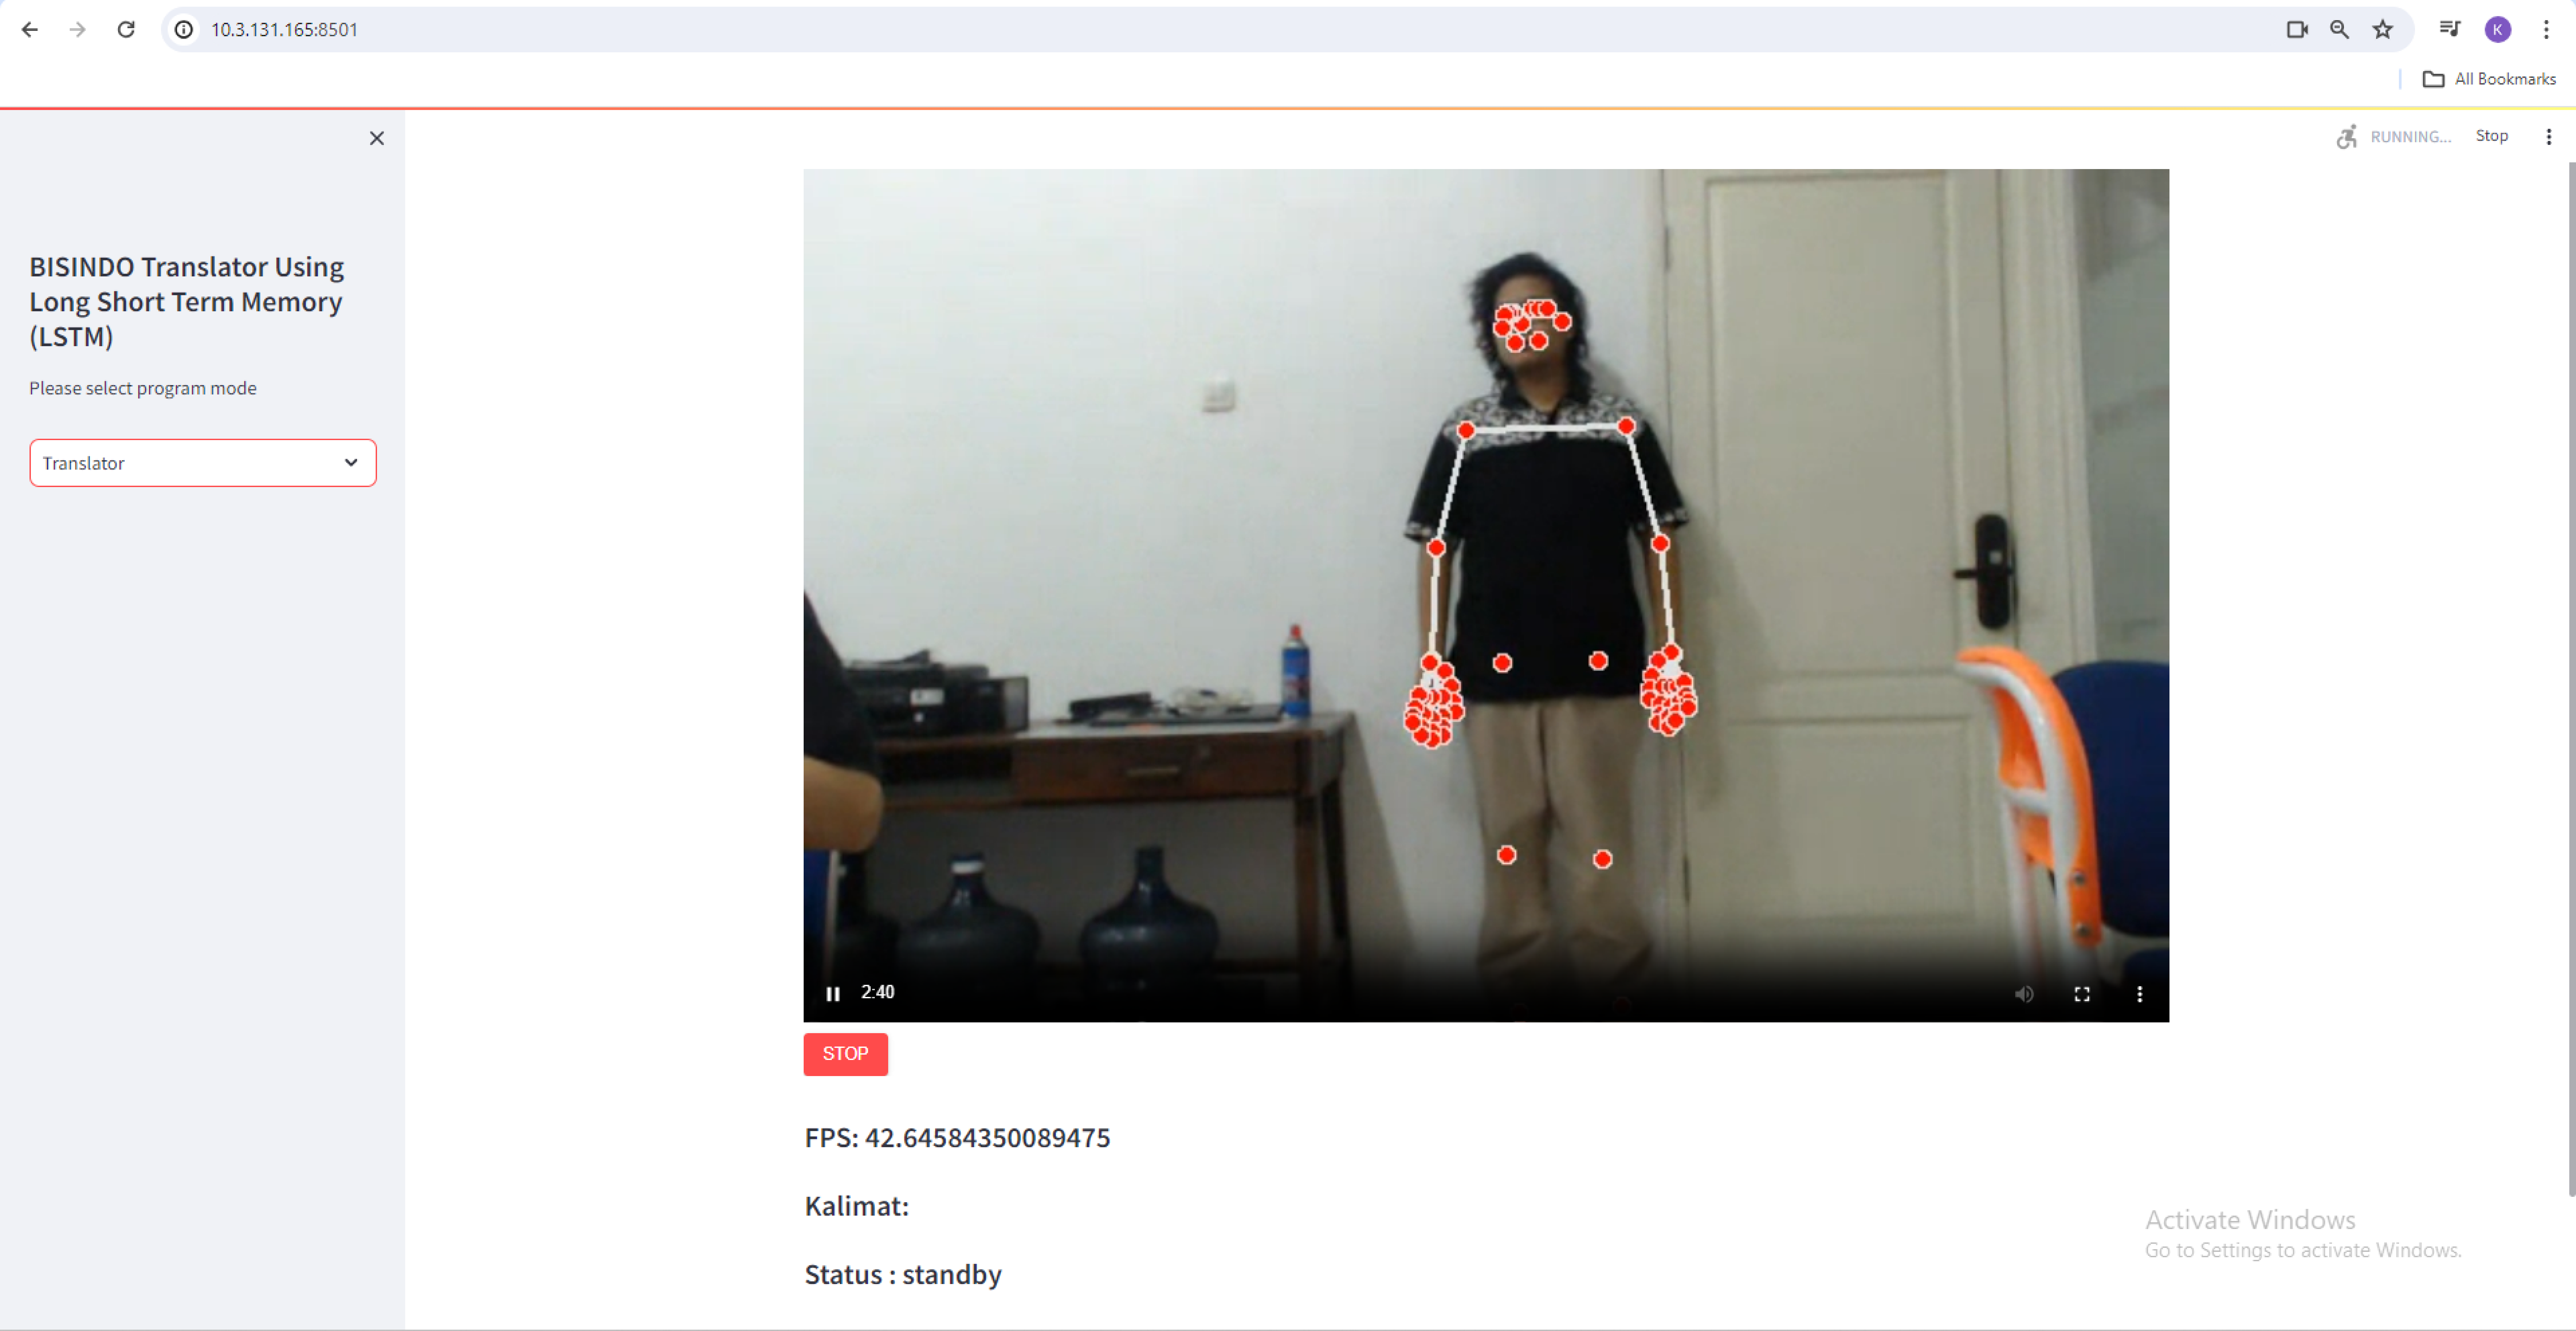
\includegraphics[scale=0.2]{gambar/bab3-layoutweb.png}

  \caption{Tampilan website}
  \label{fig:tampilanwebsite}
\end{figure}


% \subsection{Integrasi Jetson Nano}

% Sebelum dapat menggunakan Jetson Nano, terlebih dahulu mengunuh dan mengingstall NVIDIA JetPack SDK yang mencakup sistem operasi, \textit{library}, API, dan driver yang diperlukan. Proses ini melibatkan penggunaan aplikasi SDK Manager yang menyediakan antarmuka pengguna grafis untuk memudahkan penginstalan dan setup. Selanjutnya, konfigurasi perangkat keras Jetson Nano, termasuk menyediakan sumber daya listrik yang stabil, menghubungkan perangkat ke monitor melalui port HDMI, serta menyiapkan periferal lain seperti keyboard dan mouse. Untuk pengembangan yang melibatkan pengolahan citra atau video, kamera yang kompatibel juga perlu dihubungkan dan dikonfigurasi. Oleh karena Jetson Nano tidak memiliki port audio, maka digunakan USB dongle untuk dapat menyambungkan Jetson Nano dengan speaker. Kemudian dilakukan instalasi untuk setiap dependency atau \textit{library} yang dibutuhkan, seperti Python, Jupyter, TensorFlow, Keras, Pytorch, MediaPipe, Numpy, Maplotlib, dan \textit{library} lainnya. Untuk dapat menunjang performa dari Jetson Nano dalam menjalankan program, terkhususnya model penerjemah bahasa isyarat, dilakukan instalasi dan setup untuk CUDA (\textit{Compute Unified Device Architecture}) sehingga Jetson Nano dapat menggunakan GPU (\textit{Graphic Processing Unit}). 

% Untuk melakukan deploy program pendeteksi bahasa isyarat pada Jetson Nano, pada model yang telah dihasilkan sebelumnya dilakukan optimasi dengan melakukan konversi menggunakan TensorRT dan kuantisasi. Hal ini dimaksudkan untuk mengoptimalkan performa model pada Jetson Nano. Kemudian program sistem penerjemah bahasa isyarat (dalam bentuk python executable) dapat ditransfer ke Jetson Nano dengan menggunakan Git. Program siap melakukan penerjemahan bahasa isyarat BISINDO.

% \section{Urutan Pelaksanaan}

% Adapun dalam pembuatan tugas akhir ini, berikut urutan pelaksanaan penelitian yang akan dilakukan oleh penulis:

% \begin{figure}[H]
%   \centering
%   \caption{Flowchart Program Pembentukan Kalimat}
%   \label{tbl:flowchartkalimat}

%   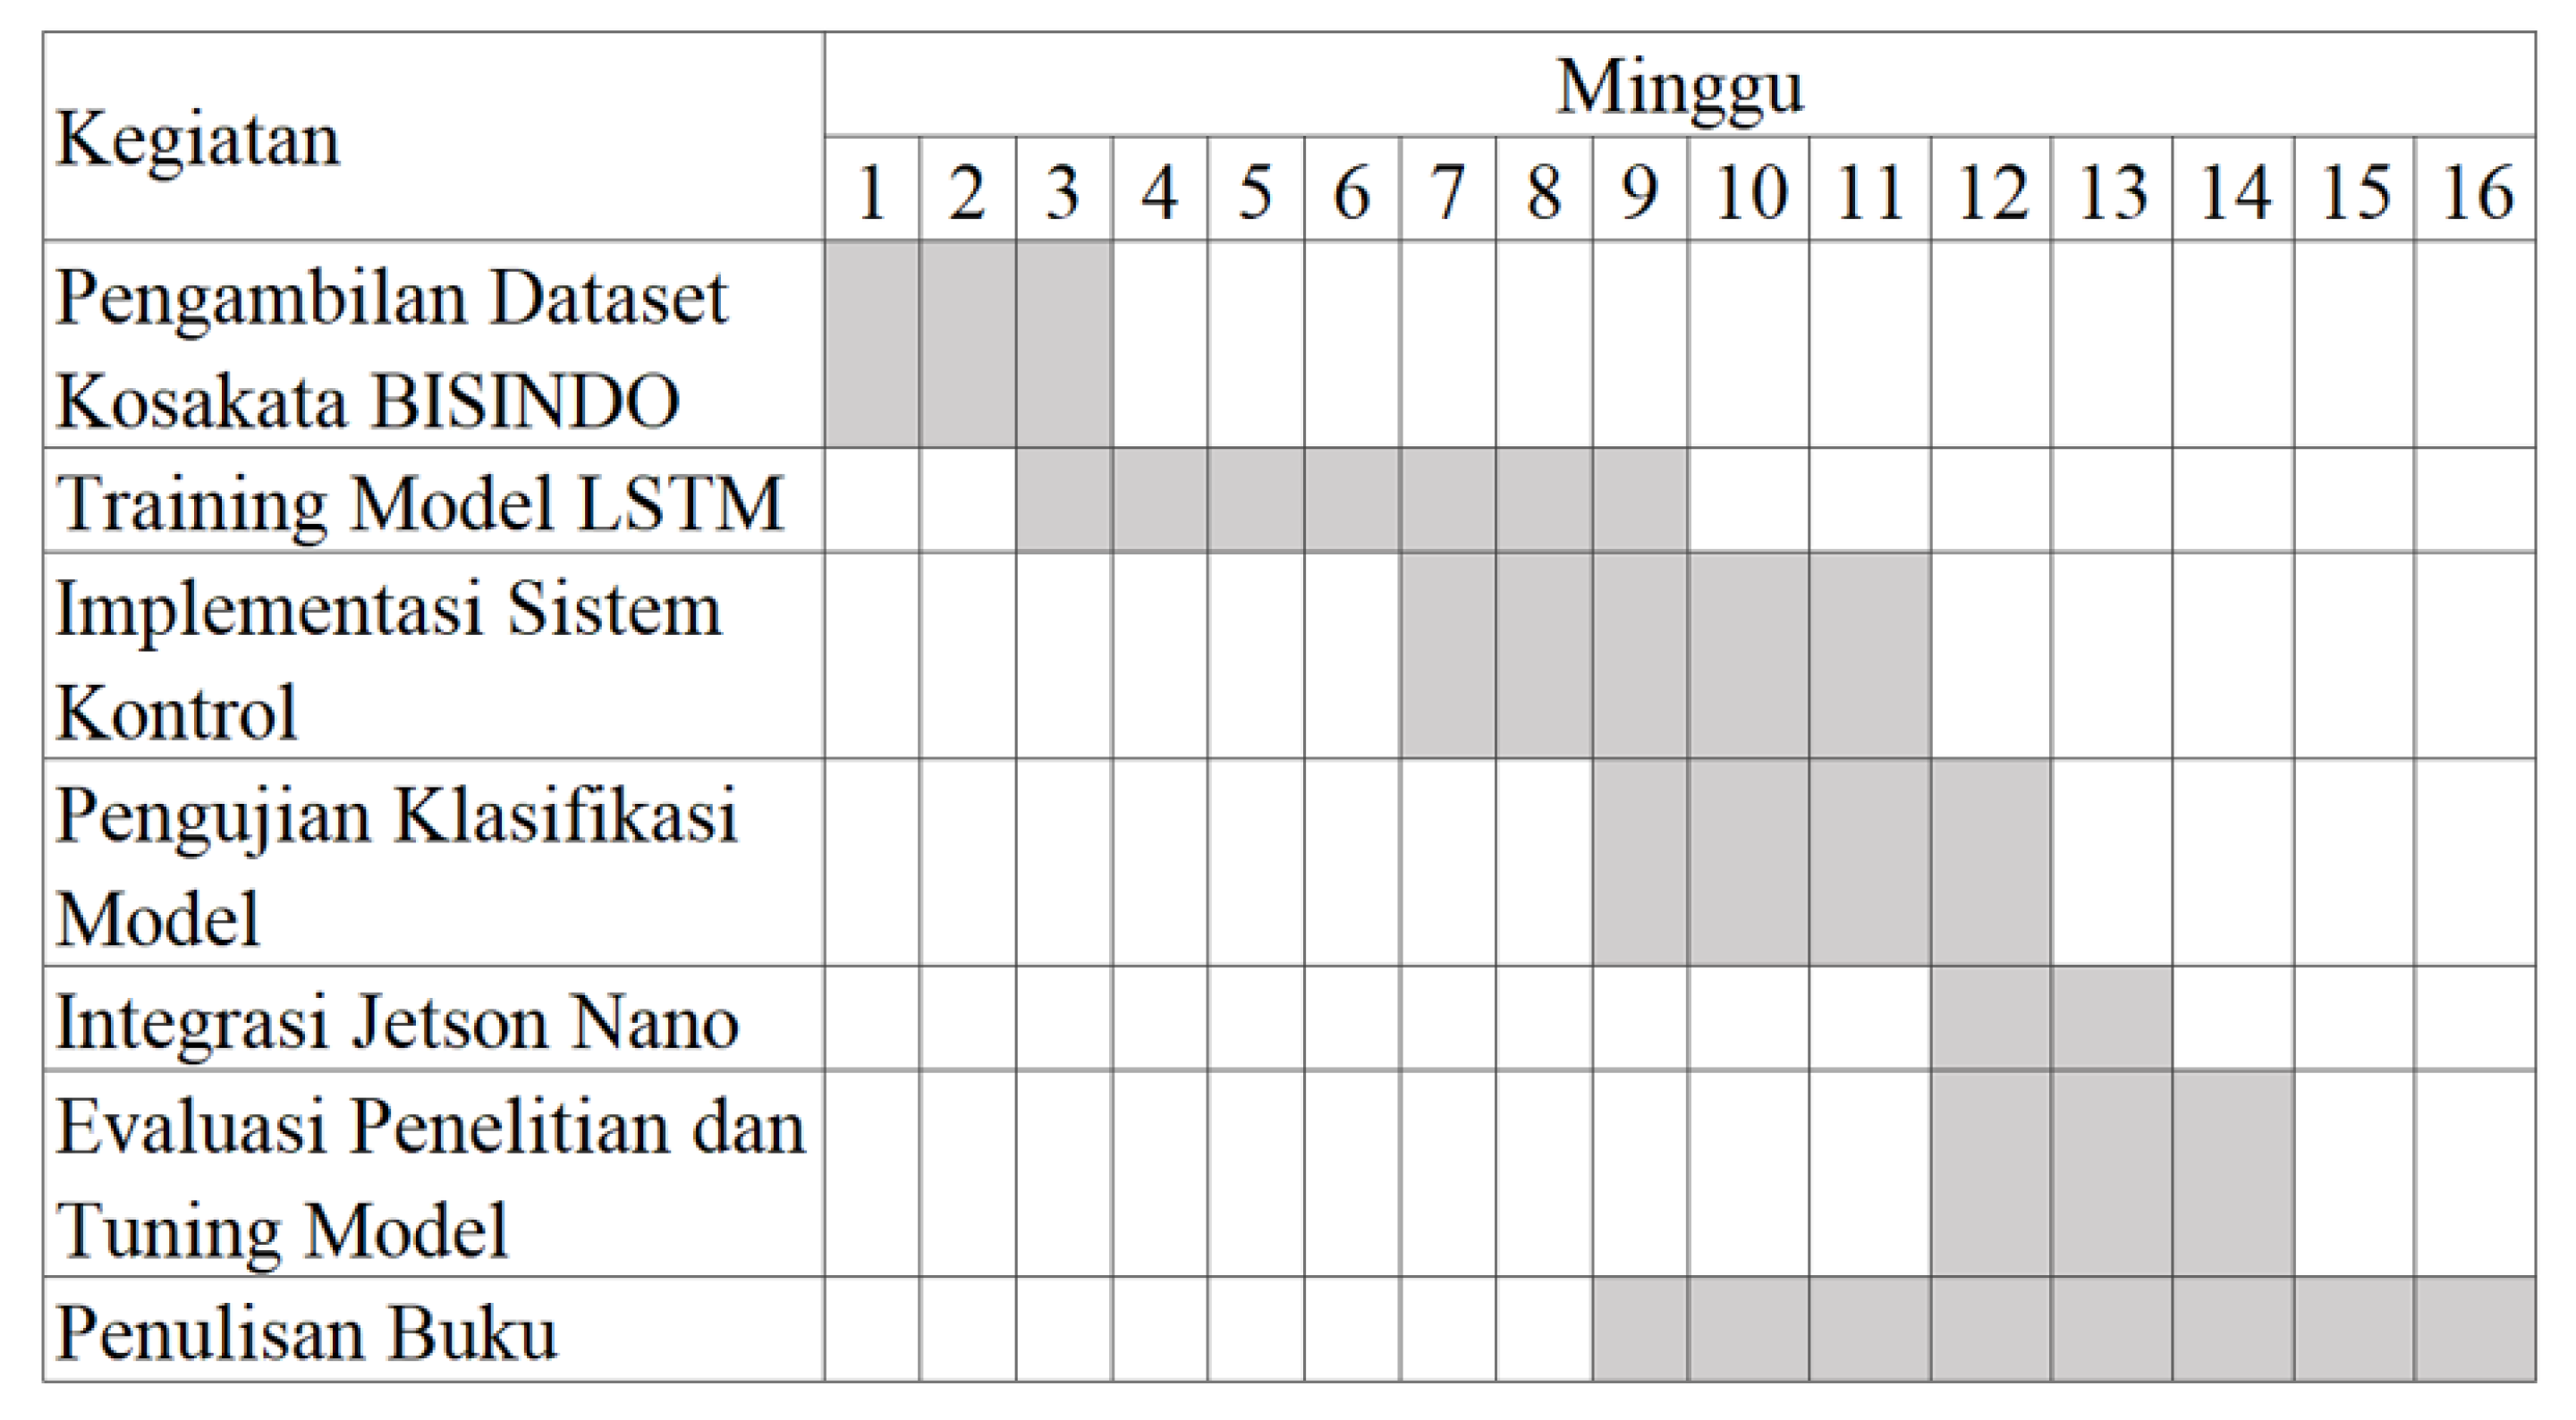
\includegraphics[scale=0.6]{gambar/bab3-timeline-kerja.png}
% \end{figure}

% \section{Deskripsi Sistem}
% \label{sec:deskripsisistem}

% Sistem akan dibuat dengan \lipsum[1-2]

% \section{Implementasi Alat
%   \label{sec:implementasi alat}}

% Alat diimplementasikan dengan \lipsum[1]

% % Contoh pembuatan potongan kode
% \begin{lstlisting}[
%   language=C++,
%   caption={Program halo dunia.},
%   label={lst:halodunia}
% ]
% #include <iostream>

% int main() {
%     std::cout << "Halo Dunia!";
%     return 0;
% }
% \end{lstlisting}

% \lipsum[2-3]

% % Contoh input potongan kode dari file
% \lstinputlisting[
%   language=Python,
%   caption={Program perhitungan bilangan prima.},
%   label={lst:bilanganprima}
% ]{program/bilangan-prima.py}

% \lipsum[4]
